\section{Visualization Pipeline}
This section details the extra code implemented in order to efficiently and effectively visualize simulation results in real time.
This is not related to the \texttt{renderppm} subcommand, which uses CPU code to render a single simulation state as an image.

\subsection{Work Scheduling}
The most important tasks are run on the GPU, and are the limiting factor for performance.
This means it's important that the GPU is running at all times.
Points where the GPU is doing no useful work are known as ``bubbles''.
% \todopending{Add figures with first 2 examples of pipeline bubbles vs. no pipeline bubbles}

To avoid these bubbles a GUI thread is spawned to prepare the current frame's draw commands and handle user input.
This runs in parallel with the simulation thread, which dispatches CUDA kernels for the simulation tick(s).
Once the sim is finished, it waits on the GUI thread (which should always be done by this point) and dispatches the draw commands through Vulkan.
It then dispatches the GUI thread again, waits for the render to finish and then immediately starts the next simulation.

\Cref{fig:CurrentSwimlane} shows the scheduling in more detail.
The GUI work can execute anywhere within the dashed lines and still not delay the final draw.
Note that the GPU is always doing useful work, and there are no bubbles.
\begin{figure}[ht]
    \centering
    \centerline{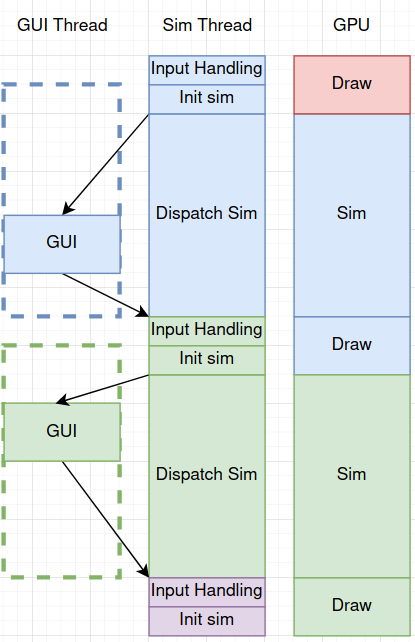
\includegraphics[width=0.5\linewidth]{ProgressReport/Ch42Design/figures/threading_usage_2.png}}
    \caption{Thread utilization diagram.}
    \label{fig:CurrentSwimlane}
    % \caption*{The GUI thread can execute anywhere within the dashed lines and still be on time.}
\end{figure}


Currently it is assumed that the rendering of one frame and the simulation of the next frame cannot happen in parallel.
\label{sec:DesignBetterScheduling}
This is also enforced by the fact that velocity and pressure buffers are used by both the simulation and the render, meaning that a simulation could not update those buffers without invoking a race condition.
However if the GPU has spare cores available while rendering a frame, then the simulation could use these cores on the next simulation at the same time.
Furthermore, most of the simulation can take place without writing to the velocity and pressure buffers, so those parts of the simulation could be run in parallel with the rendering without any worries.
Or, of course, the simulation could be double-buffered and run entirely in parallel with the rendering.

\subsection{Simulation Timing}
% \todopending{This is probably too complicated to get into fully right now. Wait until full report?}
% Define terminology: simulation time, simulation tick, real time, frame number 

% Currently the code simulates 16ms of simulation time every frame, regardless of how long it actually takes to do so.
As specified by \cref{req:VizSomeSpeed} there are two acceptable modes that the visualization can run in:
Flat Out (\cref{req:VizFlatOut}), where the simulation runs as fast as possible;
and Locked Framerate (\cref{req:VizLockedFPS}), where a frame-rate is selected and the visualization only produces that many frames per second.
The definition of a flat-out speed is that if Frame $N$ takes some amount of real-world time $t_N$, then the next frame should simulate $t_N$ seconds of simulation-time before it is presented.
This way the simulation runs as fast as possible, but it could lead to situations where if the simulation takes too long, the next simulation will have to simulate even more time and take longer etc.

With a locked frame-rate the simulation selects a timestep $\delta{t}$ to simulate for each frame, and limits the speed at which frames are produced.
If the frame-rate is 60 frames per second, then the visualization would potentially have to delay itself so that each frame takes $1/60 = \SI{16.67}{ms}$.

Currently the visualization does not take either of these approaches, but simulates a fixed $\delta{t} = 1/60$ without limiting the frame-rate.
This means on the researcher's current setup, which has a monitor capable of showing 120fps, the visualization runs 120 ticks per second which results in a simulation that's 2x faster than real-time.
This shows the simulation is fast, which is promising, but it fails the requirements.